%%%%%%%%%%%%%%%%%%%%%%%%%%%%%%%%%%%%%%%%%
% Wenneker Article
% LaTeX Template
% Version 2.0 (28/2/17)
%
% This template was downloaded from:
% http://www.LaTeXTemplates.com
%
% Authors:
% Vel (vel@LaTeXTemplates.com)
% Frits Wenneker
%
% License:
% CC BY-NC-SA 3.0 (http://creativecommons.org/licenses/by-nc-sa/3.0/)
%
%%%%%%%%%%%%%%%%%%%%%%%%%%%%%%%%%%%%%%%%%

%----------------------------------------------------------------------------------------
%	PACKAGES AND OTHER DOCUMENT CONFIGURATIONS
%----------------------------------------------------------------------------------------

\documentclass[10pt, a4paper, twocolumn]{article} % 10pt font size (11 and 12 also possible), A4 paper (letterpaper for US letter) and two column layout (remove for one column)

\usepackage[english]{babel} % English language hyphenation
\usepackage{microtype} % Better typography
\usepackage{amsmath,amsfonts,amsthm} % Math packages for equations
\usepackage[svgnames]{xcolor} % Enabling colors by their 'svgnames'
\usepackage[hang, small, labelfont=bf, up, textfont=it]{caption} % Custom captions under/above tables and figures
\usepackage{booktabs} % Horizontal rules in tables
\usepackage{lastpage} % Used to determine the number of pages in the document (for "Page X of Total")
\usepackage{graphicx} % Required for adding images
\usepackage{amssymb}
\usepackage[mathscr]{eucal}
\usepackage[table]{xcolor}
\usepackage{enumitem} % Required for customising lists
\setlist{noitemsep} % Remove spacing between bullet/numbered list elements
\usepackage{sectsty} % Enables custom section titles
\allsectionsfont{\usefont{OT1}{phv}{b}{n}} % Change the font of all section commands (Helvetica)
\usepackage{hyperref}
\usepackage[sort,numbers]{natbib}
%----------------------------------------------------------------------------------------
%	MARGINS AND SPACING
%----------------------------------------------------------------------------------------
\usepackage{geometry} % Required for adjusting page dimensions
\geometry{
	top=0.65cm, % Top margin
	bottom=1.5cm, % Bottom margin
	left=1.5cm, % Left margin
	right=1.5cm, % Right margin
	includehead, % Include space for a header
	includefoot, % Include space for a footer
	%showframe, % Uncomment to show how the type block is set on the page
}
\setlength{\columnsep}{6mm} % Column separation width


%----------------------------------------------------------------------------------------
%	FONTS
%----------------------------------------------------------------------------------------

\usepackage[T1]{fontenc} % Output font encoding for international characters
\usepackage[utf8]{inputenc} % Required for inputting international characters
\usepackage{XCharter} % Use the XCharter font

%%%%%%%%%%%%%%%%%%%%%%%%%%%%%%%%%%%%%%%%%%
% Wenneker Article
% Structure Specification File
% Version 1.0 (28/2/17)
%
% This file originates from:
% http://www.LaTeXTemplates.com
%
% Authors:
% Frits Wenneker
% Vel (vel@LaTeXTemplates.com)
%
% License:
% CC BY-NC-SA 3.0 (http://creativecommons.org/licenses/by-nc-sa/3.0/)
%
%%%%%%%%%%%%%%%%%%%%%%%%%%%%%%%%%%%%%%%%%

%----------------------------------------------------------------------------------------
%	PACKAGES AND OTHER DOCUMENT CONFIGURATIONS
%----------------------------------------------------------------------------------------

\usepackage[english]{babel} % English language hyphenation

\usepackage{microtype} % Better typography

\usepackage{amsmath,amsfonts,amsthm} % Math packages for equations

\usepackage[svgnames]{xcolor} % Enabling colors by their 'svgnames'

\usepackage[hang, small, labelfont=bf, up, textfont=it]{caption} % Custom captions under/above tables and figures

\usepackage{booktabs} % Horizontal rules in tables

\usepackage{lastpage} % Used to determine the number of pages in the document (for "Page X of Total")

\usepackage{graphicx} % Required for adding images

\usepackage{enumitem} % Required for customising lists
\setlist{noitemsep} % Remove spacing between bullet/numbered list elements

\usepackage{sectsty} % Enables custom section titles
\allsectionsfont{\usefont{OT1}{phv}{b}{n}} % Change the font of all section commands (Helvetica)

%----------------------------------------------------------------------------------------
%	MARGINS AND SPACING
%----------------------------------------------------------------------------------------

\usepackage{geometry} % Required for adjusting page dimensions

\geometry{
	top=1cm, % Top margin
	bottom=1.5cm, % Bottom margin
	left=2cm, % Left margin
	right=2cm, % Right margin
	includehead, % Include space for a header
	includefoot, % Include space for a footer
	%showframe, % Uncomment to show how the type block is set on the page
}

\setlength{\columnsep}{7mm} % Column separation width

%----------------------------------------------------------------------------------------
%	FONTS
%----------------------------------------------------------------------------------------

\usepackage[T1]{fontenc} % Output font encoding for international characters
\usepackage[utf8]{inputenc} % Required for inputting international characters

\usepackage{XCharter} % Use the XCharter font

%----------------------------------------------------------------------------------------
%	HEADERS AND FOOTERS
%----------------------------------------------------------------------------------------

\usepackage{fancyhdr} % Needed to define custom headers/footers
\pagestyle{fancy} % Enables the custom headers/footers

\renewcommand{\headrulewidth}{0.0pt} % No header rule
\renewcommand{\footrulewidth}{0.4pt} % Thin footer rule

\renewcommand{\sectionmark}[1]{\markboth{#1}{}} % Removes the section number from the header when \leftmark is used

%\nouppercase\leftmark % Add this to one of the lines below if you want a section title in the header/footer

% Headers
\lhead{} % Left header
\chead{\textit{\thetitle}} % Center header - currently printing the article title
\rhead{} % Right header

% Footers
\lfoot{} % Left footer
\cfoot{} % Center footer
\rfoot{\footnotesize Page \thepage\ of \pageref{LastPage}} % Right footer, "Page 1 of 2"

\fancypagestyle{firstpage}{ % Page style for the first page with the title
	\fancyhf{}
	\renewcommand{\footrulewidth}{0pt} % Suppress footer rule
}

%----------------------------------------------------------------------------------------
%	TITLE SECTION
%----------------------------------------------------------------------------------------

\newcommand{\authorstyle}[1]{{\large\usefont{OT1}{phv}{b}{n}\color{DarkRed}#1}} % Authors style (Helvetica)

\newcommand{\institution}[1]{{\footnotesize\usefont{OT1}{phv}{m}{sl}\color{Black}#1}} % Institutions style (Helvetica)

\usepackage{titling} % Allows custom title configuration

\newcommand{\HorRule}{\color{DarkGoldenrod}\rule{\linewidth}{1pt}} % Defines the gold horizontal rule around the title

\pretitle{
	\vspace{-30pt} % Move the entire title section up
	\HorRule\vspace{10pt} % Horizontal rule before the title
	\fontsize{32}{36}\usefont{OT1}{phv}{b}{n}\selectfont % Helvetica
	\color{DarkRed} % Text colour for the title and author(s)
}

\posttitle{\par\vskip 15pt} % Whitespace under the title

\preauthor{} % Anything that will appear before \author is printed

\postauthor{ % Anything that will appear after \author is printed
	\vspace{10pt} % Space before the rule
	\par\HorRule % Horizontal rule after the title
	\vspace{20pt} % Space after the title section
}

%----------------------------------------------------------------------------------------
%	ABSTRACT
%----------------------------------------------------------------------------------------

\usepackage{lettrine} % Package to accentuate the first letter of the text (lettrine)
\usepackage{fix-cm}	% Fixes the height of the lettrine

\newcommand{\initial}[1]{ % Defines the command and style for the lettrine
	\lettrine[lines=3,findent=4pt,nindent=0pt]{% Lettrine takes up 3 lines, the text to the right of it is indented 4pt and further indenting of lines 2+ is stopped
		\color{DarkGoldenrod}% Lettrine colour
		{#1}% The letter
	}{}%
}

\usepackage{xstring} % Required for string manipulation

\newcommand{\lettrineabstract}[1]{
	\StrLeft{#1}{1}[\firstletter] % Capture the first letter of the abstract for the lettrine
	\initial{\firstletter}\textbf{\StrGobbleLeft{#1}{1}} % Print the abstract with the first letter as a lettrine and the rest in bold
}

%----------------------------------------------------------------------------------------
%	BIBLIOGRAPHY
%----------------------------------------------------------------------------------------

\usepackage[backend=bibtex,style=authoryear,natbib=true]{biblatex} % Use the bibtex backend with the authoryear citation style (which resembles APA)

\addbibresource{example.bib} % The filename of the bibliography

\usepackage[autostyle=true]{csquotes} % Required to generate language-dependent quotes in the bibliography
 % Specifies the document structure and loads requires packages

%----------------------------------------------------------------------------------------
%	ARTICLE INFORMATION
%----------------------------------------------------------------------------------------
\begin{document}



\title{$\mathcal{ROBHOOT}$ \\ Open Research Network \\ Whitepaper v.1.0} % The article title
  \author{XX{\textsuperscript{1,2,3} and XY\textsuperscript{2,3}} % Authors
  \newline\newline % Space before institutions
  \\
	\textsuperscript{1}\institution{}\\ % Institution 1
	\textsuperscript{2}\institution{}\\ % Institution 2
	%\textsuperscript{3}\institution{\texttt{LaTeXTemplates.com}}
      %} % Institution 3


% Example of a one line author/institution relationship
%\author{\newauthor{John Marston} \newinstitution{Universidad Nacional Autónoma de México, Mexico City, Mexico}}

\date{\today} % Add a date here if you would like one to appear underneath the title block, use \today for the current date, leave empty for no date
%---------------------------------------------------------------------------------------

%\begin{document}

\maketitle % Print the title
\thispagestyle{firstpage} % Apply the page style for the first page (no headers and footers)

%----------------------------------------------------------------------------------------
%	ABSTRACT
%----------------------------------------------------------------------------------------
\lettrineabstract{\section{{\bf Summary}} Robhoot aims to fully
  automate the research cycle in a open decentralized
  network. Research automation with reporting generation might help to
  contrast informed decisions when solving complex social,
  environmental and technological problems. Current technologies for
  scientific inquiry and decision-making are highly fragmented and
  thus only increase robustness, reproducibility, open-access and the
  interactions with the public marginally. The goal of Robhoot is to
  propose a hybrid-neutral-technology to lay out the foundation for an
  open-science research ecosystem aiming to strengthen the robustness
  and reproducibility of science. Robhoot is not set out to deliver a
  finished research open network in the science ecosystem, but to
  provide a science-enabled technology in establishing a prototype
  proof-of-principle to connect automated, decentralized and
  neutral-knowledge generation with knowledge-inspired societies.}
%----------------------------------------------------------------------------------------
%	ARTICLE CONTENTS
%----------------------------------------------------------------------------------------
\section{The Science Ecosystem}
The process of science and technology requires multiple steps of
information transfer among trusted/untrusted peers. Science and
technology produce knowledge and features like reproducibility,
decentralization, and immutability of knowledge are key to reach
neutral open-access reports when taking informed decisions in complex
social, environmental and technological problems. However, currently
public funded science is highly centralized
\citep{Inhaber1977,Gunther2018}⁠⁠, prone to errors \citep{Fang2011},
difficult to reproduce \citep{Hardwicke2018}, and contains many biases
\citep{Ioannidis2005}. In this regard, automated-based knowledge
following a secure peer-to-peer architecture storing the open-source
knowledge graphs derived from the paths of the research cycle is far
from reality. Taken together, these elements make the connection
between the scientific process, open-access and reproducible research
reporting for decision-making highly improbable. Despite many projects
are aiming at making the science ecosystem less centralized and biased
while increasing openness and reproducibility a science-enabled
technological paradigm connecting open-science to knowledge-inspired
societies is not currently in place \citep{Gunther2018}.

Many studies in decentralized ecosystems are producing an immense gain
in detailed knowledge about scalability, security and decentralization
trade-offs
\citep{Golem2016,Durov2017,Androulaki2018,OceanProtocolFoundation2018,BigchainDBGmbH2018}. Automation
and AI technologies is the other angle from which many advances are
rapidly occurring \citep{Schmidhuber:2015,Reichstein,Gil2019}. Yet,
while the existing technological paradigm is rapidly shifting towards
science-based decentralization and automation technologies, end-to-end
open-source research accounting for decentralized, neutral and
automated knowledge-inspired technologies are missing (Table 1). Rapid
advances of automated research platforms facilitating data integration
accounting for part of the research cycle are currently under
development\footnote{This is by no means an exhaustive list but it
  gives an indication of the many projects currently in place:
  \href{https://www.nterminal.com}{NakamotoT},\href{https://cloud.google.com/bigquery/}{BigQuery},\href{https://www.automaticstatistician.com/index/}{Automated
    statistician},\href{http://www.modulos.ai/}{Modulos},\href{https://ai.google/}{Google
    AI},\href{https://iris.ai}{Iris},\href{https://github.com/DS3Lab/easeml}{easeml}}
but open-source decentralized and automated networks accounting fully
for the research cycle are still at a very incipient stage of
development. While conceptual frameworks conceptualizing the required
layers in many research fields are well established (Figure 1a), there
is currently a lack of integration, development and automated tools
connecting knowledge graphs (Figure 1b) to deep process-based learning
networks to explore their robustness (Figure 1c) in fully
decentralized ecosystems (Figure 1d).

\begin{table}
 %\rowcolor{pink}
\begin{tabular}{ p{3cm} | p{2cm} | p{2cm}}
  \hline \hline
  \textbf{Features} & \textbf{Science Ecosystem} &\textbf{Robhoot 1.0}\\  \hline
  Decentralization & No & Yes \\ \hline
  Open-access & Mostly No & Yes \\ \hline
  Immutability & No & Yes \\ \hline
  Robustness & Mostly No & Yes \\ \hline
  Reproducibility & Mostly No & Yes \\ \hline        
  Owner-Controlled assets & No & Yes \\ \hline       
  \bottomrule

\end{tabular}
\caption{Robhoot aims to be designed to resolve desirable properties
  of science: Robustness, Reproducibility, Decentralization, Open and
  Direct access to reporting by peers and not-peers.}
\end{table}
% ------------------------------------------------
  \section{Robhoot Design Goals}
  Robhoot will be developed in four different stages following
  standard version protocols. The most advanced version is to provide
  real-time open-access reporting by a decentralized neutral-knowledge
  network to gain informed decisions when solving complex social,
  environmental and technological problems. Automating the research
  cycle in a open research network ultimately aims to contrast
  human-produced science with machine-produced science to enrich the
  human-knowledge graphs in a neutral-knowledge-inspired
  society. Figures 1 to 3 show Robhoot stages, Robhoot in a digital
  ecosystem and the timeline for each of the stages, respectively.
  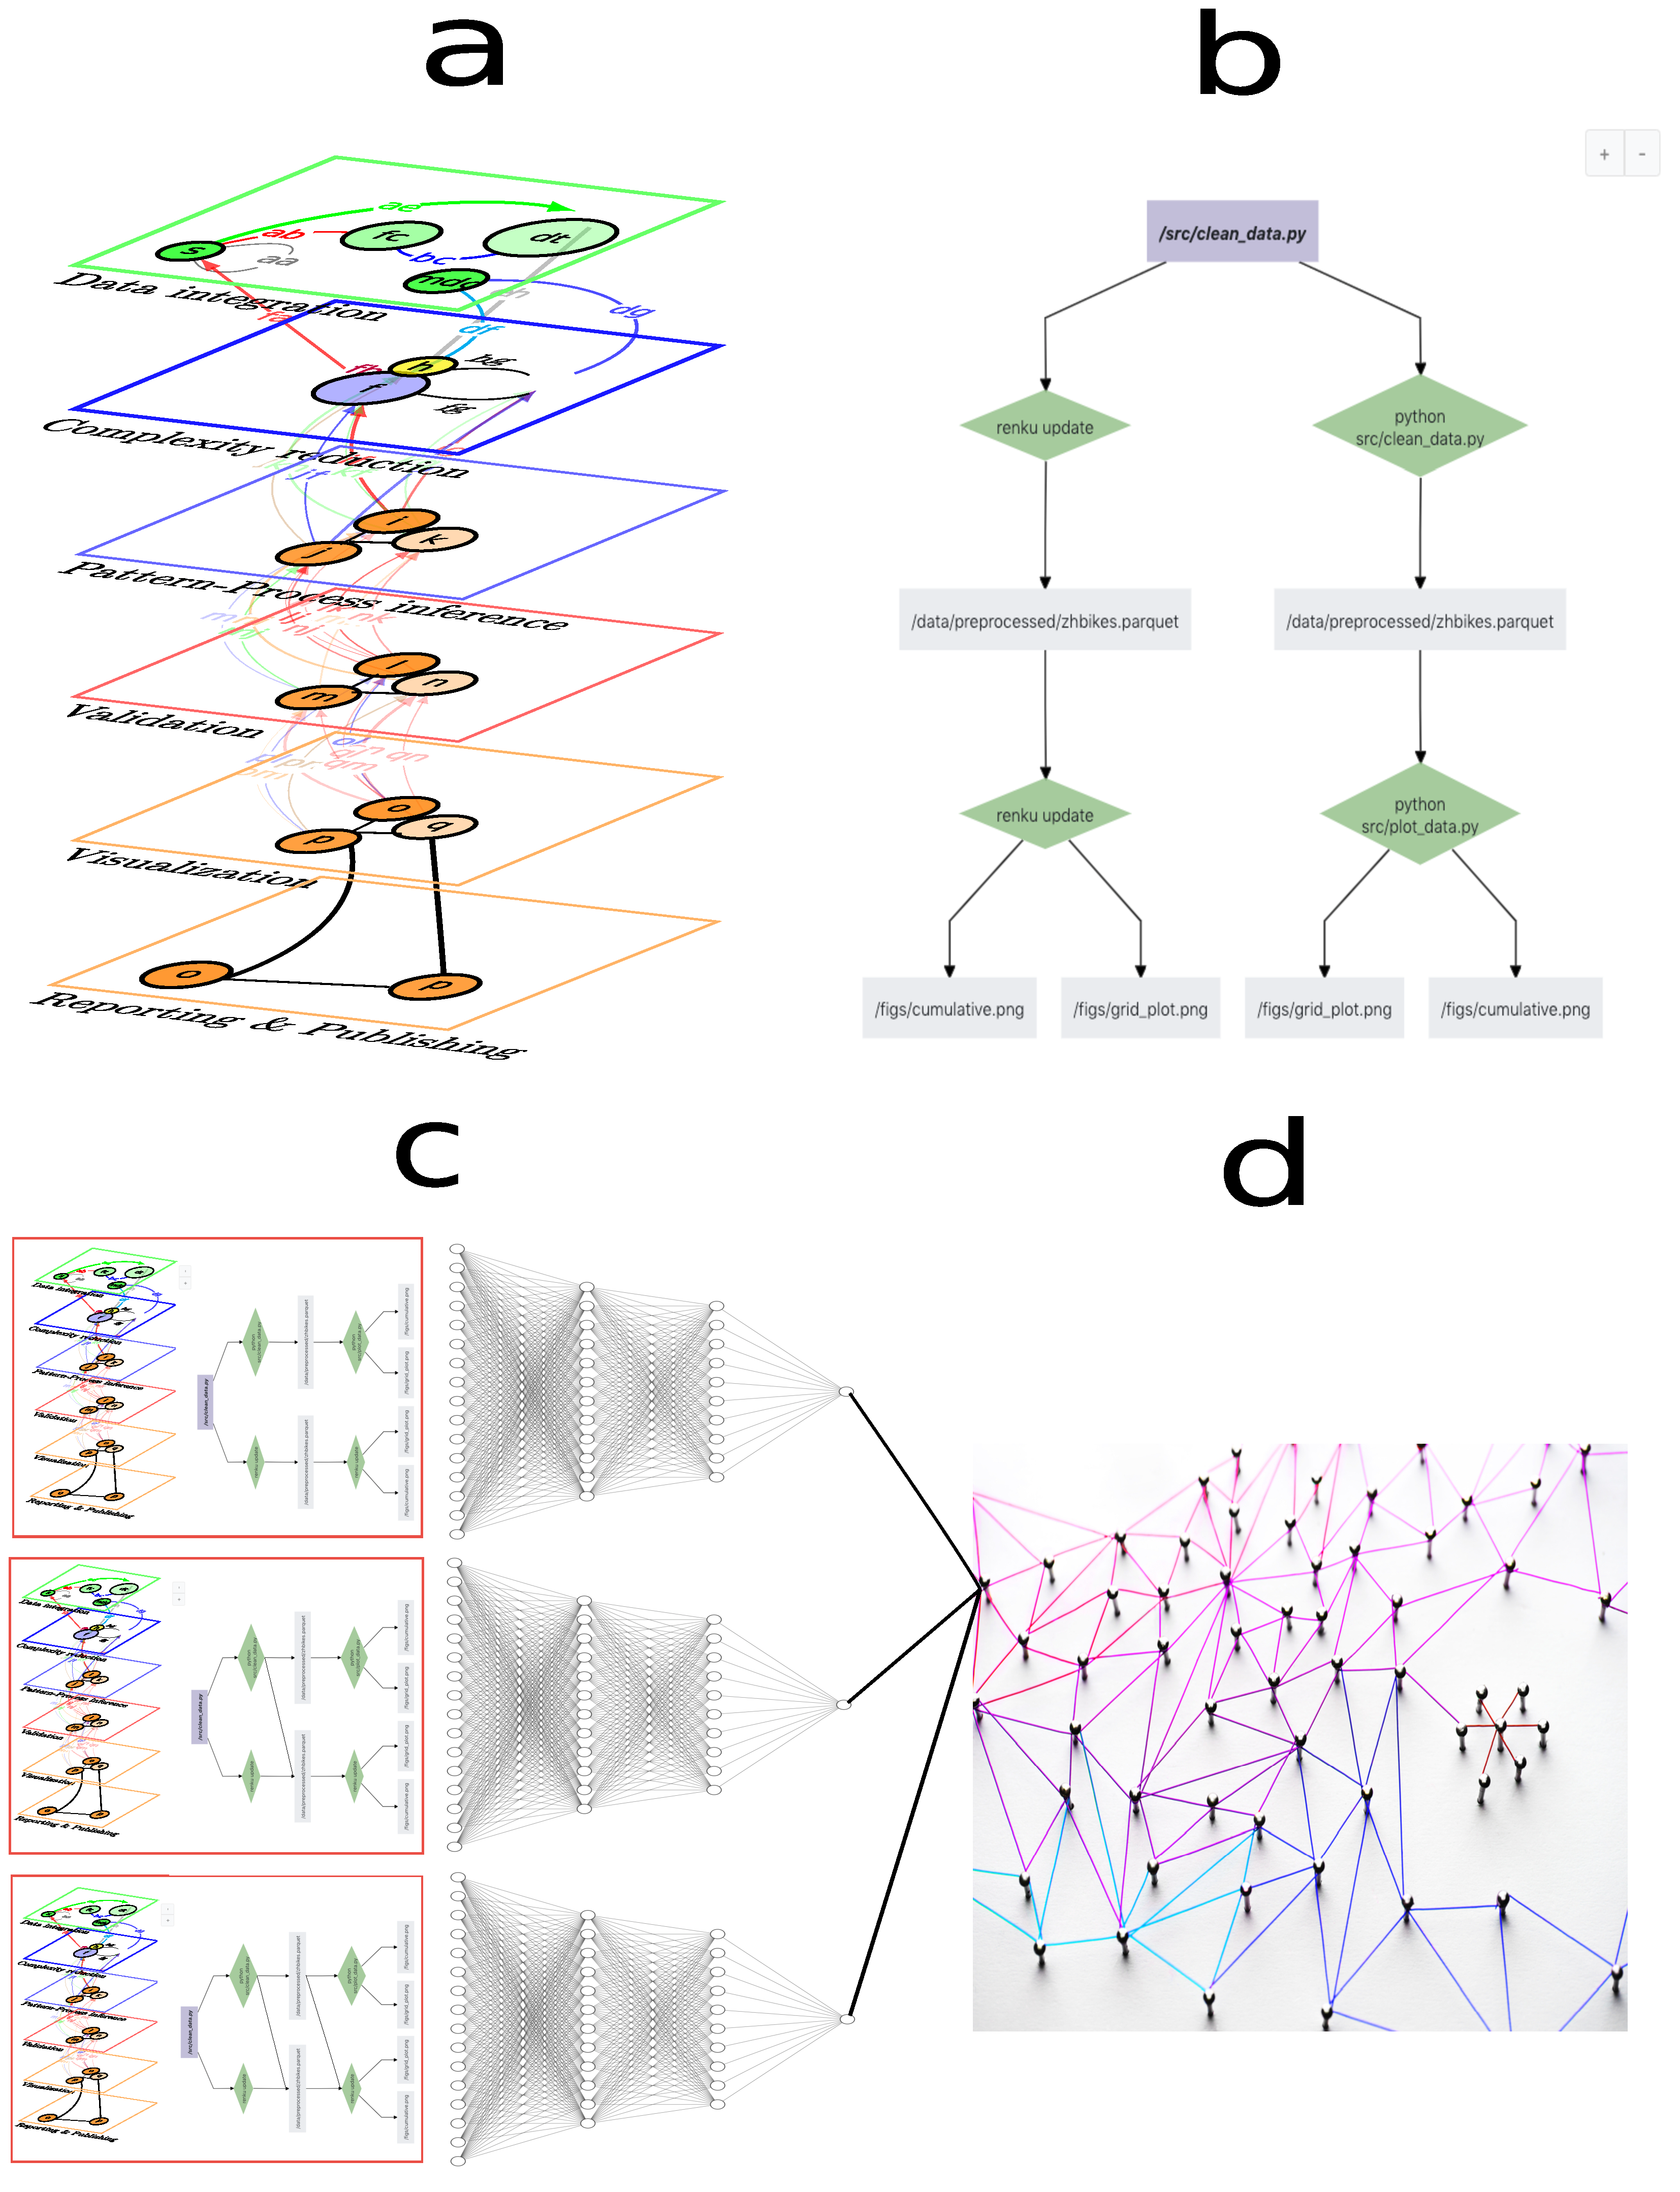
\includegraphics[width=0.45\textwidth]{Figure1.pdf}

  %\begin{figure*}[ht]
  {\small {\bf Figure 1: Automated knowledge-based network
      technology}. {\bf a}) {\bf Robhoot 1.0} will account fully for
    the research cycle from data integration (top) to reporting
    generation (bottom). {\bf b}) {\bf Robhoot 2.0} will encode each
    path of the research cycle in {\bf a} as a knowledge graph
    (KG). {\bf c}) {\bf Robhoot 3.0} will add deep knowledge-based
    networks to automatically explore populations of KGs to gain
    robustness of the process-based patterns contained in the
    data. {\bf d}) {\bf Robhoot 4.0} will deploy all KGs in a
    distributed network of mutually trusting/untrusting peers with
    every peer maintaining the population of the KGs.}
  %\end{figure*}
  
  The overall objectives and a brief numeration of the tools and
  methods to be used/developed in each stage for each of the four
  major Robhoot versions are the following:
  \vspace{-0.15 in}
  \subsection{Robhoot 1.0: Automated Research Cycle}
   \begin{itemize}
   \item Develop, deploy and integrate open-source algorithms to
     fully automate the research cycle (Figure 1a).
   \item Exploration of robustness within and between layers from data
     integration, complexity reduction, inference, and validation to
     visualization and automated reporting (Figure 1a).
   \item Robhoot 1.0 testnet to explore a Open Research Network in
     Biodiversity and Global Change Research to connect open science
     (i.e., citizen and other data-driven models) to real-time
     open-access knowledge generation to gain informed decisions when
     solving local and global environmental problems.
   \end{itemize}

   \begin{itemize}
   \item {\bf Tools and Methods}: Multilayer networks, Bayesian
     Networks, Network metrics, Julia computing language, Open-source
     software protocols, Gitchain, ETLs algorithms, Kafka, Clickhouse.
 \end{itemize}
 \vspace{-0.15 in}
   
  \subsection{Robhoot 2.0: Knowledge Graphs}
  \begin{itemize}
  \item Implementation of algorithms to reproduce paths of the
    research cycle with Knowledge Graphs (KGs) (Figure 1b).
  \item Robustness and stability exploring a suite of open-source
    lineage client-tracker algorithms.
  \end{itemize}

   \begin{itemize}
   \item {\bf Tools and Methods}: Knowlegde graph algorithms and
     packages (i.e., Renku and others).
 \end{itemize}
  \vspace{-0.15 in}
  
  \subsection{Robhoot 3.0: Deep learning networks}
  \begin{itemize}
  \item Deploy automated deep learning algorithms to sample paths of
    the research cycle to produce populations of Knowledge Graphs
    (KGs) (Figures 1a-c).
  \item Exploration of the robustness of automated research cycle combining
    optimization algorithms and the population of Knowledge Graphs
    (Figure 1c).
  \end{itemize}

 \begin{itemize}
 \item {\bf Tools and Methods}: Multilayer networks, Neural Biological
   Networks, Bayesian Networks, Deep learning networks. Optimization
   algorithms.
 \end{itemize}
  
  \vspace{-0.15 in}
  
  \subsection{Robhoot 4.0: Distributed ledger network}
  \begin{itemize}
  \item Deploy a permissioned-permissionless distributed ledger
    technology to guarantee decentralization, open-access,
    neutral-knowledge-based network and prior
    confidenciality/posterior reproducibility of the KGs populations
    (Figures 1c and 1d).
  \item Exploration of a suite of consensus algorithms and smart
    contracts among trusted-untrusted peer-to-peer interactions to
    infer macroscopic metrics of the open research network (Figure
    1d).
  \item Quantification of metrics to study the
    scalability-security-decentralization trade-offs when storing KGs
    in the research network (Figure 1d).
  \item Testnet case study to explore the interaction between
    consensus protocols and the scalability-security-decentralization
    trade-offs when committing the KGs to the distributed ledger.
  \item Mainnet to cryptographically link each population of KGs to
    previous KGs-ledger to create an historical KGs-ledger chain that
    goes back to the genesis ledger in the open research network. The
    mainnet aims to connect multiple database with real-time
    open-access citizen data science to knowledge-inspired societies.
  \end{itemize}

   \begin{itemize}
   \item {\bf Tools and Methods}: Distributed computing algorithms,
     Blockchain and consensus algorithms, BighainDB,
     Gitchain. Telegram open network, Golem.
 \end{itemize}
  
  \section{Robhoot in Digital Ecosystems}
  The science ecosystem currently lack technologies fully automating
  the research cycle into digital ecosystems. Despite public
  institutions are demanding more reproducibility and openness of the
  data and the scientific process, and overall a shifting towards open
  and reproducible scientific and engineering landscapes, there are
  not currently open and integrated technologies aiming to compactly
  facilitate and distribute the scientific and engineering knowledge
  in open, reproducible and immutable knowledge networks.
  
  Automating knowledge-generation requires the integration of many
  distinct traits or features. Usually, knowledge-generation comes
  from interactions within- and between-layers of the scientific
  process (Figure 1a). The feedbacks occurring among layers in the
  science and technology ecosystem also provide unexpected behaviors
  that are difficult to anticipate. Therefore many feedbacks and
  interactions within- and between-layers are not easy to reproduce if
  not properly accounted for. Robhoot will take advantage of the
  open-source software community to explore how knowledge graphs,
  optimization, automation, and decentralization algorithms can be
  connected to the robustness and reproducibility of the scientific
  process.

  Therefore, Robhoot aims to be a hybrid-technology accounting for
  many traits (Table 1: decentralized, open-access, immutable, robust,
  reproducible, and secure with trusted/untrusted peer-to-peer
  interactions). Producing such a multitrait technology means
  multidisciplinarity teams compactly making functional interactions
  within a rapidly evolving digital ecosystem. In this regard, Robhoot
  aims to put together scientists and engineers from data science,
  computer science (i.e., distributed computing, software
  development), the physics of complex systems (i.e., multilayer
  networks), artificial intelligence (i.e., deep learning and
  automation) and the biology, ecology and evolution of social,
  natural and technological ecosystems.

  One way of visualizing the multitrait dimensionality of Robhoot in
  the digital ecosystem is to connect each layer of the scientific
  process (Figure 1a) to the open-source software required to gain
  functionality of the automated research cycle (Figure 2). For
  example, Node 0 (left column, Figure 2) can be the Data Integration
  layer (Figure 1a). This node is connected to seven nodes that might
  represent open-source ETLs (i.e., extract, transform, load data
  open-source software, central column, Figure 2). Connections between
  Node 0 and nodes 5, 6, 8, 9, 10, 12 and 13 might be rapidly evolving
  (i.e., indicated by the different red tones of the
  connections). Indeed, open-source ETLs are rapidly evolving towards
  accounting for many heterogeneous aspects of data integration (i.e.,
  formats, historical-real time, storage, dimensions, size, bias and
  spatiotemporal resolution). ETLs might also be connected to a
  gradient of reporting generation (i.e., right column, Figure 2)
  noting reports containing only a subset of the interactions of the
  digital ecosystem network. The network of the fully automated
  research cycle can be one where Nodes 0, 1, 2, 3, and 4 represent
  the different layers of the research cycle (left column, Figure 2
  and Figure 1a) connected to the open-source software of the digital
  ecosystem (central column, Figure 2) to produce the full population
  of reports (right column, Figure 2).


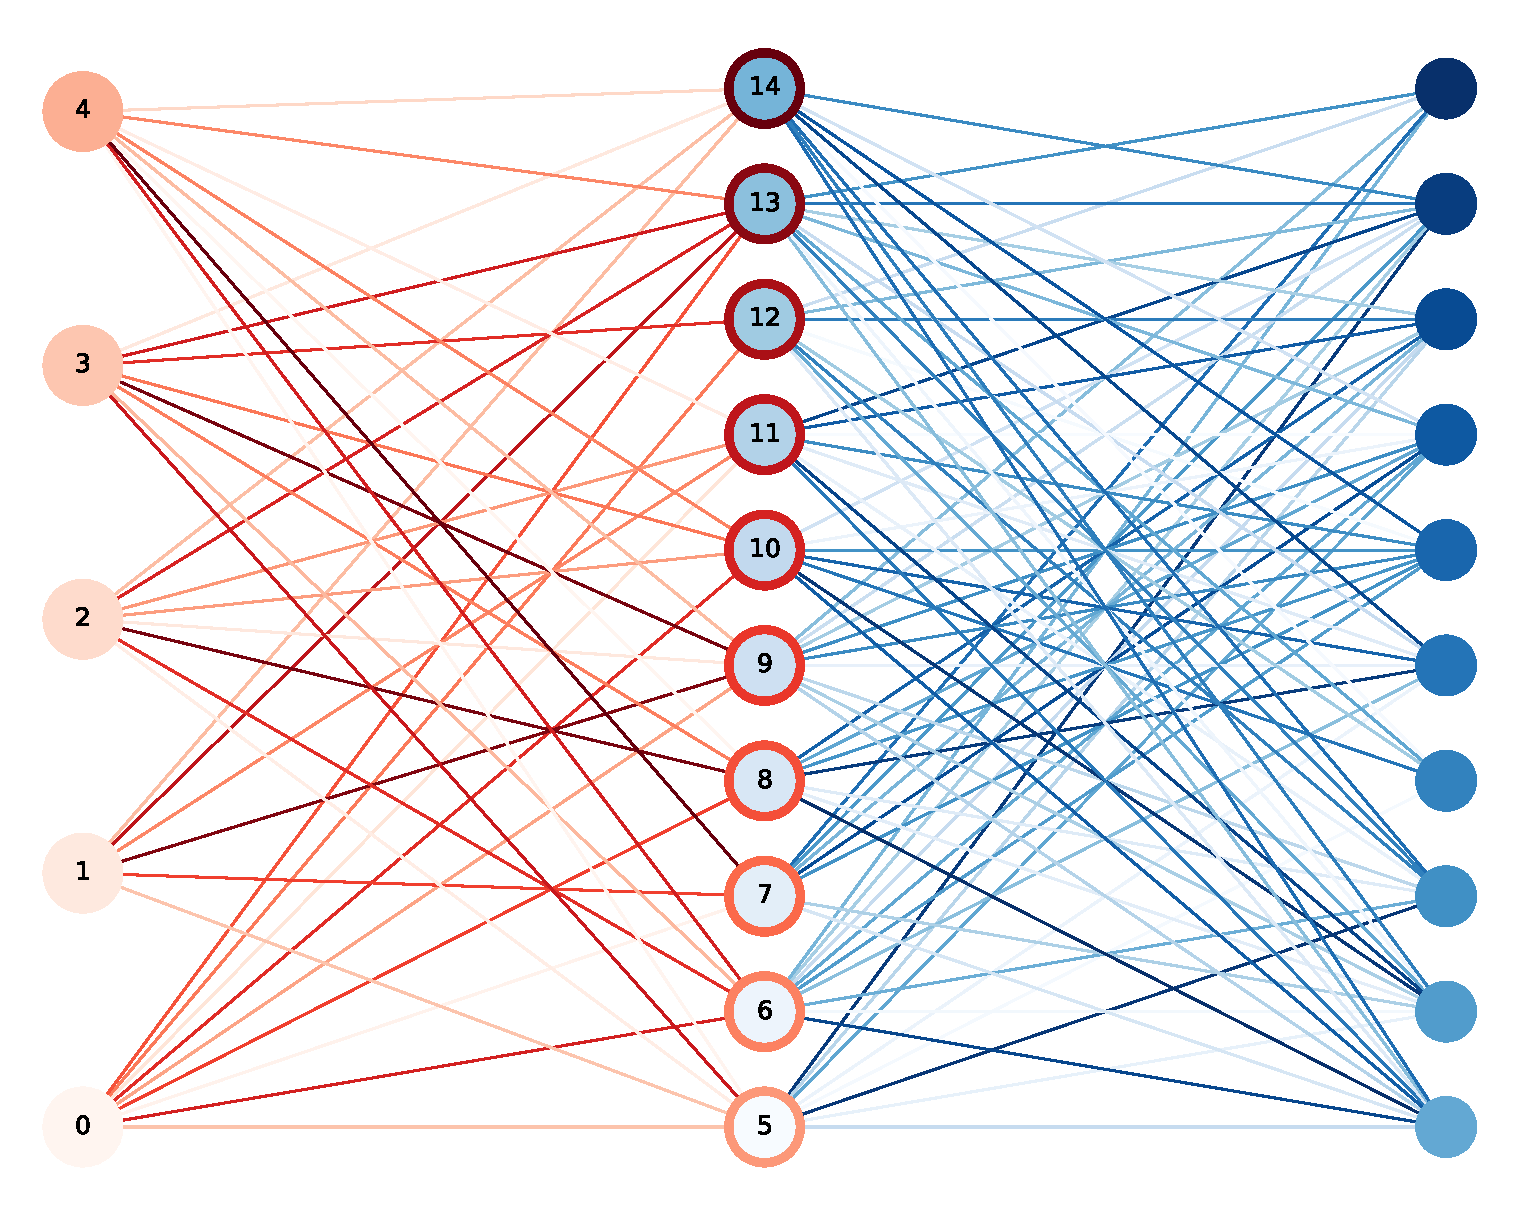
\includegraphics[width=0.45\textwidth]{FigureRobhoot.pdf}

%\begin{figure*}[ht]
{\small {\bf Figure 2: Robhoot in Digital Ecosystems}: {\bf Left
    column}: {\bf Robhoot 1.0} containing the research cycle
  represented as nodes (i.e., from node 0 to 4: Data integration (0),
  Complexity Reduction (1), Inference (2), Validation (3), and
  Visualization(4)). {\bf Central column}: The research cycle layers
  connected to the open-source software in the digital
  ecosystem. Nodes can for example represent the ETLs open-source
  software required to produce a general data integration accounting
  for many data heterogeneities. {\bf Right column}: Reporting
  gradient connected to the open-source software where each report
  (i.e., represented as a node) is generated only using a subset of
  the research layers and ETLs.}
%\end{figure*}


%\section{How to contribute to Robhoot}

%\section{The Robhoot roadmap}
%The following is a first version of the roadmap, the backbone from
%where a more detailed FET-EU proposal will be generated.

\begin{figure*}[ht]
  \centering 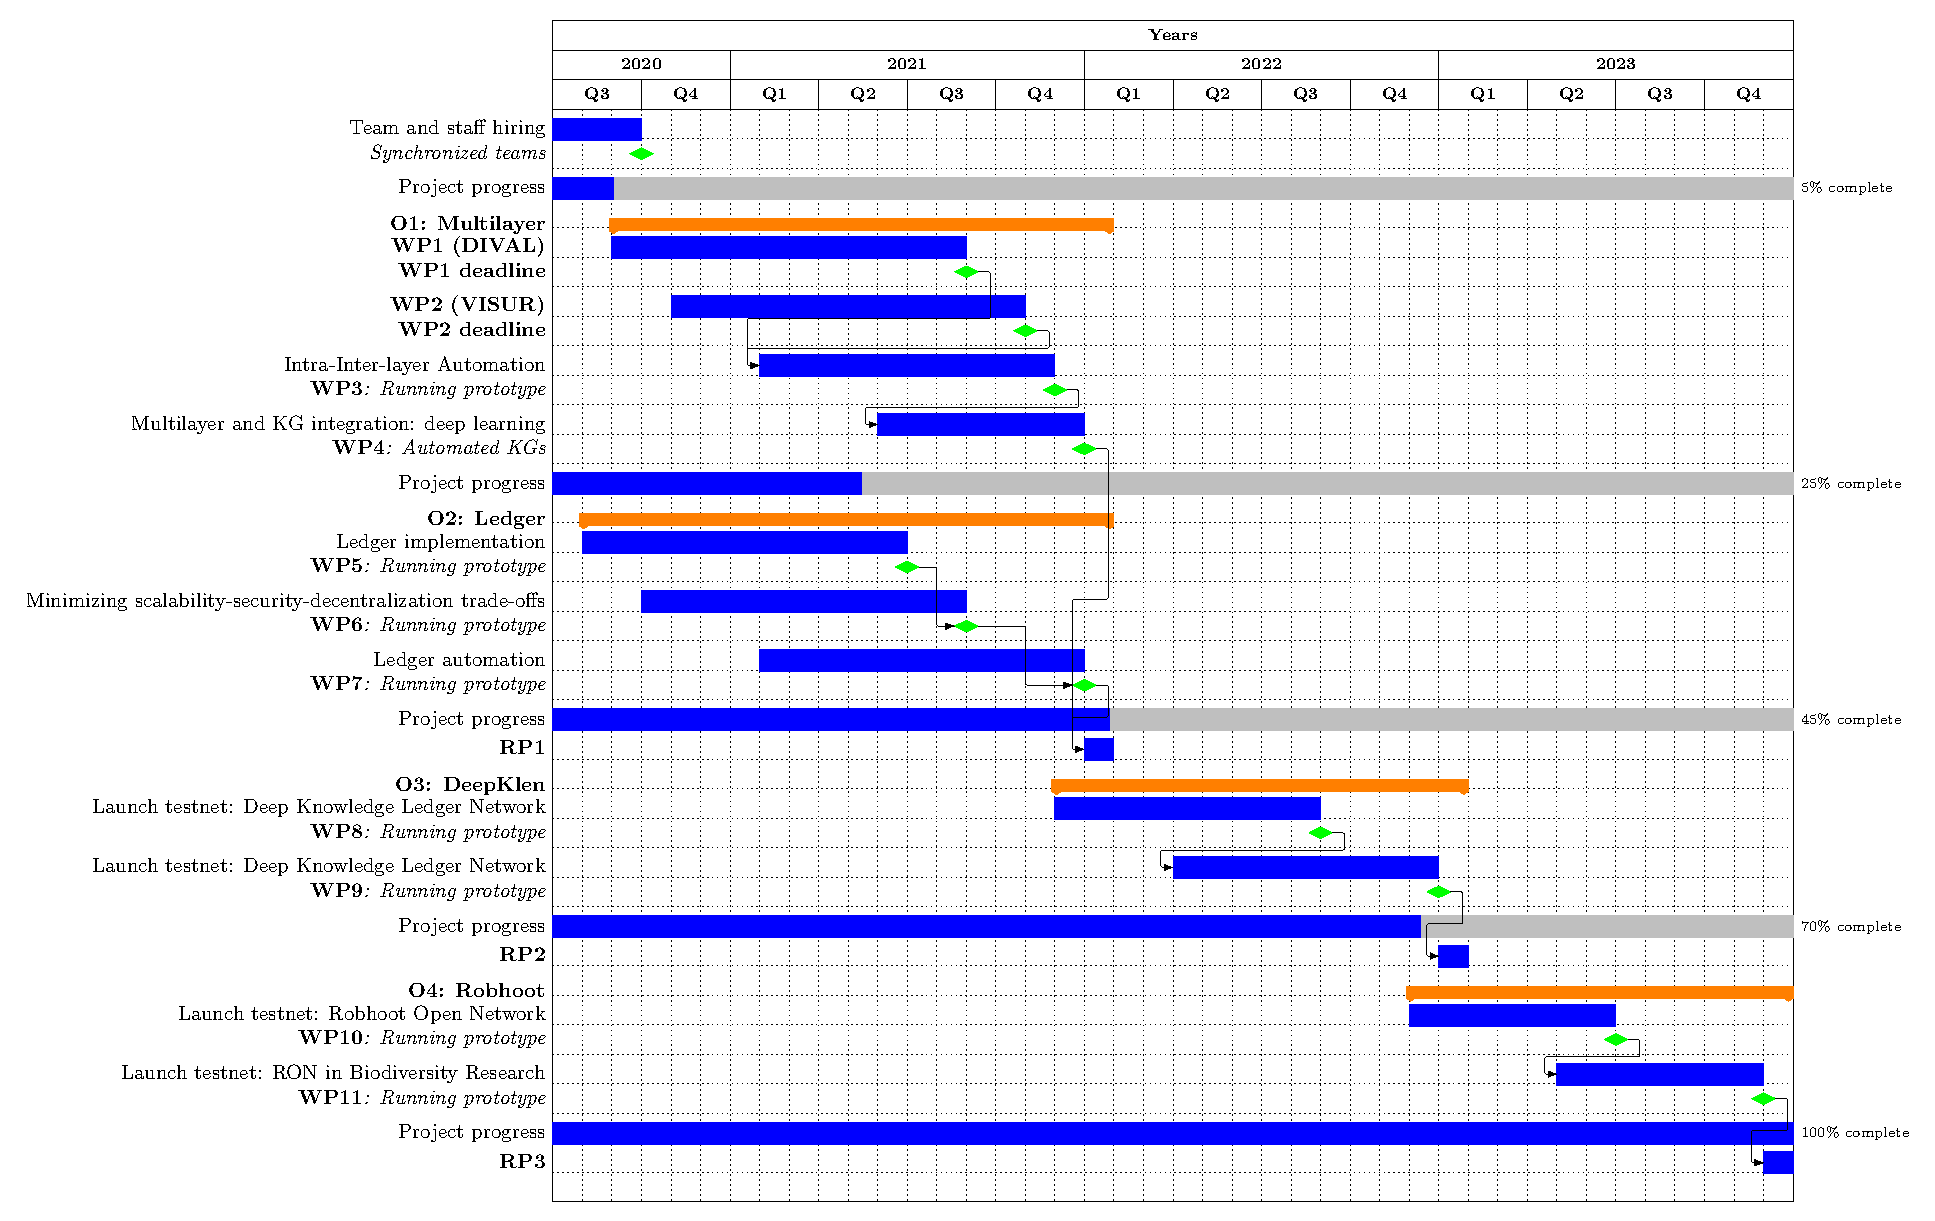
\includegraphics[width=1\textwidth]{GanttChart.pdf}
  {\small {\bf Figure 3: The Robhoot roadmap}: {\bf Robhoot 1.0}
    working packages {\bf WP1} to {\bf WP4}: Develop, integrate,
    deploy and test the functionality of interacting open-source
    algorithms to fully automate the research cycle (Figure 1a). {\bf
      Robhoot 2.0} working packages {\bf WP5} to {\bf WP7}: Fully
    automate end-to-end research cycle exploring, implementing an
    testing knowledge graphs. {\bf Robhoot 3.0} working packages {\bf
      WP8} to {\bf WP11}: Developing, implementing and testing deep
    knowledge-based networks to automatically explore populations of
    KGs to gain robustness of the process-based patterns contained in
    the data. {\bf Robhoot 4.0} working packages {\bf 12} to {\bf 13}:
    Deploy all KGs in a distributed network of mutually
    trusting/untrusting peers with every peer maintaining the
    population of the KGs.}
\end{figure*}


%\newpage
\section{Conclusion}
Science and technology ecosystems are in need of accounting for the
uncertainties, reproducibility and immutability related to the
complexity of the research process. This need is not just for a
specific stage of the research cycle, but from data acquisition and
integration to automated reporting generation because
knowledge-inspired societies and decentralized governance will demand
full research cycle transparency to solve complex social,
environmental and technological problems. This need brings many
challenges to our research proposal because obtaining robust knowledge
from integrating many layers of the research cycle, each containing
its own set of methods and uncertainties, can generate divergent,
fragile and contradictory outcomes.

We will develop a flexible research method focusing step by step in
different stages with varying levels of complexity (i.e., from Robhoot
1.0 to 4.0, Figure 3). Our motivation will be to provide a first
open-access proof of concept of how the technology works: we will
automate reproducible research paths along a multilayer network
(Robhoot 1.0) to sample the KGs (Robhoot 2.0) using different deep
learning algorithms to estimate the uncertainty of the ruled-based
inference obtained by fitting predictions to simulated data (Robhoot
3.0). Accounting for the uncertainties of each of the research stages
when sampling the KGs comes from the many distinct paths within and
across the layers in the research cycle (Figure 1a). Robhoot will test
a variety of consensus algorithms to explore the degree of security,
decentralization and scalability of the ledger knowledge network using
the generated population of KGs (Robhoot 4.0).

Despite our focus will be bias towards the algorithmic robustness
during the four stages of Robhoot development, we will develop a
domain-specific case study, a Robhoot Open Network, to test the
robustness of the rule-based inference obtained by fitting each of the
generated KG to empirical patterns. The high risk associated to
robustly automate the full research cycle for producing immutable open
knowledge will be buffered to a great extend because the existing
digital ecosystem of highly reliable open-source software tools
(Figure 2).

%----------------------------------------------------------------------------------------
%	BIBLIOGRAPHY
%----------------------------------------------------------------------------------------

%\printbibliography[title={Bibliography}] % Print the bibliography, section title in curly brackets

%\newpage
\bibliographystyle{unsrtnat}
%\bibliographystyle{tree.bst}
\bibliography{Robhoot.bib}

%----------------------------------------------------------------------------------------

\end{document}

\hspace{-0.2 in}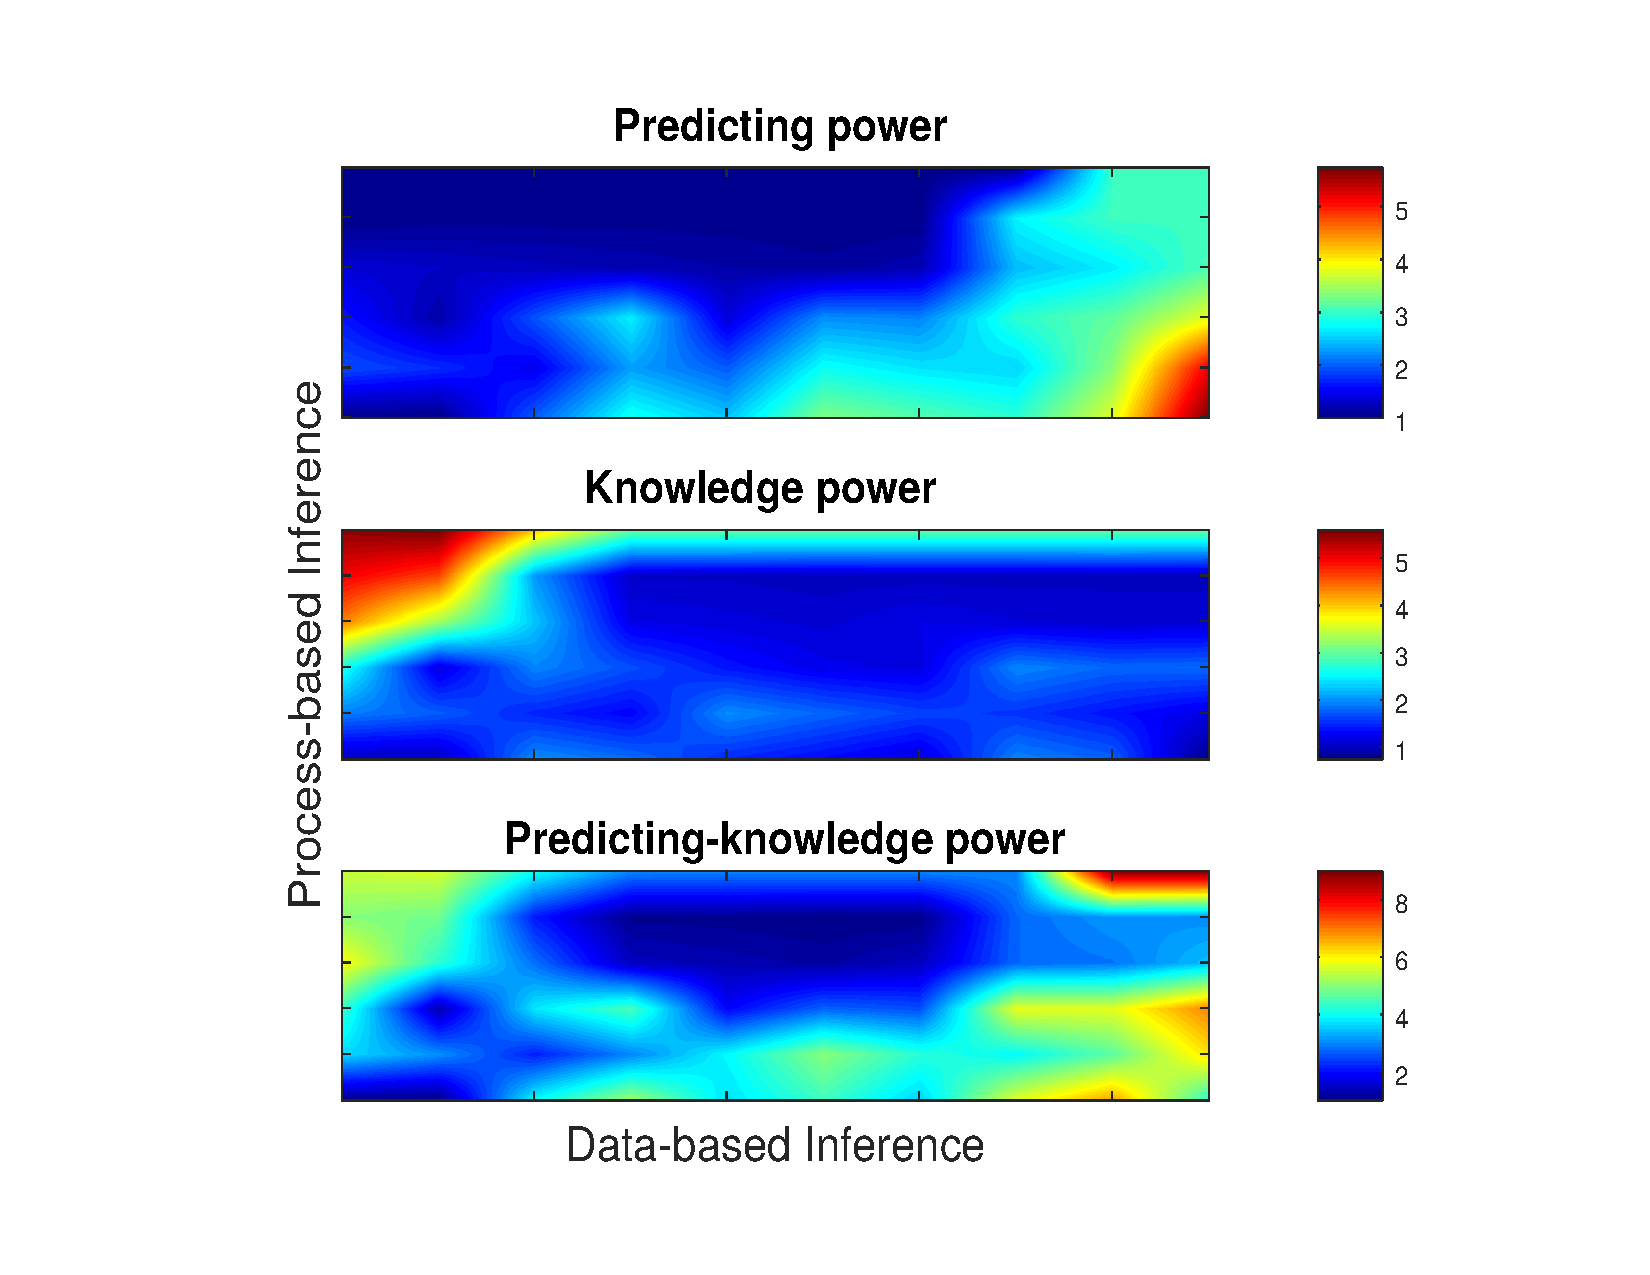
\includegraphics[width=0.52\textwidth]{Figure3.pdf}
{\small {\bf Figure 1: Prediction power (top), understanding (middle),
    and prediction-understanding power maps (bottom)}. x-axis
  represents data-based inference (i.e., gradient of AI methods from
  low (left) to high (right) predictive power). y-axis represents
  process-based inference (i.e., gradient of process-based methods
  from low (bottom left) to high (top left) understanding power). The
  gradient of predicting power map (top) shows a hot spot red area in
  the bottom right highlighting the region where AI methods best
  predict the empirical data. The gradient of understanding power map
  (middle) shows a red hot spot in the top left highlighting the
  region where the best mechanistic understanding occur. The
  predicting-understanding power map (bottom) shows the sum of the two
  previous maps highlighting a red hot spot where the best synthesis
  research joining predicting and understanding power of the empirical
  data might occur. The first research goal of this proposal aims to
  build an automated research platform to maximize the predicting and
  understanding power highlighted in the red hot spot of the
  predicting-understanding power map (bottom).}
